\chapter{Identification of Transfer Function of a Single Board Heater System through Ramp Response Experiment}\label{chap2}
The aim of this experiment is to perform ramp test on a Single Board Heater System and to identify system transfer 
function using ramp response data. The target group is anyone who has basic knowledge of control engineering.

\begin{figure}
\centering
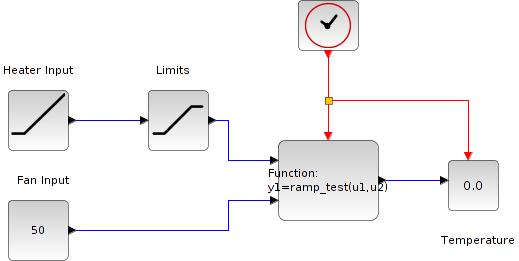
\includegraphics[width=0.7\linewidth]{Ramp-test_manual/ramp_test.jpg}
\caption{Xcos for ramp test experiment}
\label{Xcos_rt}
\end{figure} 

\begin{figure}
\centering
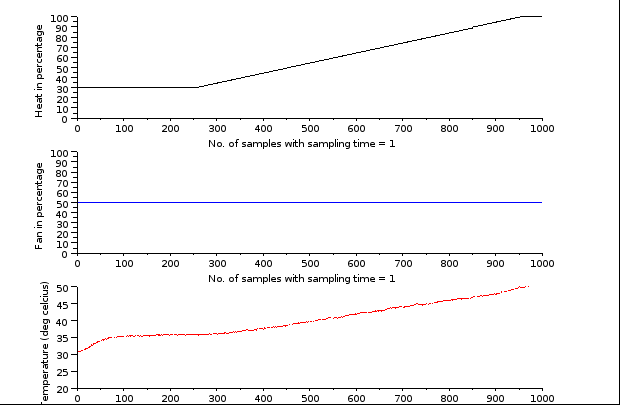
\includegraphics[width=\linewidth]{Ramp-test_manual/ramp-test.png}
\caption{Screen shot of ramp test experiment}
\end{figure}

We have used Scilab and Xcos as an interface for sending and receiving data. 
Xcos diagram is shown in figure \ref{Xcos_rt}. Heater current and fan speed are the two inputs for this system. 
They are given in percentage of maximum. These inputs can be varied by setting the properties of the input block's properties 
in Xcos. The plots of their amplitude versus number of collected samples are also available on the scope windows. 
The output temperature profile, as read by the sensor, is also plotted. The data acquired in the process is stored on the 
local drive and is available to the user for further calculations.

 In the {\tt ramp\_test.xcos} file, open the heater block's parameters to give a ramp input to the system with some value for slope. For this experiment, we have chosen slope = $0.1$. Double click on the ramp input block labled as {\tt Heater input}. Change the following values in the respective fields: slope = 0.1, start time = 200, initial output = 20. Keep the fan constant at 100.


\begin{table}
\begin{verbatim}
1.0      30.0      50.0       28.1   1416462726532.0
2.0       30.0        50.0         28.1   1416462727574.0
.
999.0         100.0       50.0        47.6   1416463723533.0
1000.0        100.0      50.0       47.6   1416463724533.0
\end{verbatim}
\caption{Ramp data obtained after performing local Step Test}
\label{rampdata}
\end{table}

The ramp test data file will be saved in {\tt Ramp\_Test} folder. The name of the file will be the date and time at which the experiment was conducted. A sample data file is provided in the same folder. The sample data file is named as {\tt ramp-data-local.txt} and {\tt ramp-data-virtual.txt}. Refer to the one depending on wheather you are performing a local or a virtual experiment. Referring to the data file thus obtained as shown in table \ref{rampdata}, the first column in this table denotes samples. The second column in this table denotes heater in percentage. It starts at 30 and increases with a step size of 10 units. The third column denotes the fan in percentage. It has been held constant at 50 percent. The fourth column refers to the value of temperature. The fifth column denotes time stamp. The virtual data file will have four time stamp columns apart from first 3 columns. These four time stamp columns are client departure, server arrival, server departure and client arrival. These can be used for advanced control algorithms. These additional time stamps exist in virtual mode because of the presense of network delay.

\section{Conducting Ramp Test on SBHS locally}
The detailed procedure to perform a local experiment is explained in Chapter\ref{sercomm}. A summary of the same is provided in section \ref{local-summary} It is same for this section with following changes.

\begin{enumerate}
\item Step1: The working directory is {\tt  Ramp\_test}
\item Step2: Same
\item Step3: Same
\item Step4: Same
\item Step5: Load ramp test function by executing command\\ {\tt exec<space>ramp\_test.sci}
\item Step6: Load Xcos code for ramp test using the command\\ {\tt exec<space>ramp\_test.xcos}
\item Step7: Same
\end{enumerate}
\section{Conducting Ramp Test on SBHS, virtually}
The detailed procedure to perform a local experiment is explained in Chapter\ref{virtual}. A summary of the same is provided in section \ref{vlabsexpt}. It is same for this section with following changes.

\begin{enumerate}
\item Step1: The working directory is {\tt  RampTest}. Open this directory.
\item Step2: Same
\item Step3: Same
\item Step4:  Switch to the RampTest experiment directory and double-click on the file {\tt ramptest.sce}. This will launch scilab and also open the file {\tt ramptest.sce} in the scilab editor. Linux users will have to launch scilab manually. They also have to change the working directory to {\tt  RampTest} and then open the {\tt  RampTest} file in the scilab editor.
\item Step5: Same
\item Step6: Execute the file {\tt ramptest.sce}.  Expect the ramp test xcos diagram to open automatically. If this doesnt happen, check the scilab console for error message.
\item Step7: Execute the ramptest xcos diagram.
\item Step8: Same
\end{enumerate}


 The virtual experiment response is shown in figure \ref{ramp-virtual}. The corresponding data file is shown in table \ref{rampdata}. The time stamps shown are cut short for better viewing. This data file can be found in {\tt RampTest} folder for virtual experiments. The name of this file is {\tt step-data-virtual.txt}.


\begin{figure}
\centering
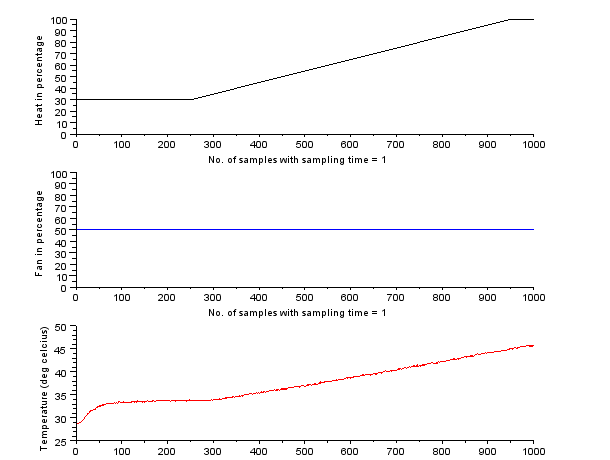
\includegraphics[width=\linewidth]{Ramp-test_manual/ramp-virtual-plot.png}
\caption{Ramp test Virtual experiment response}
\label{ramp-virtual}
\end{figure}


\begin{table}
\begin{verbatim}
0 0 100 28.80 14...8993 14...0301 14...0318 14...9040 0.10000E+01
1 30 50 28.80 14...2861 14...4172 14...4189 14...2908 0.10000E+01
.
.
617 66 50 39.10 14...7141 14...8476 14...8494 14...7188 0.61700E+03
618 66 50 39.10 14...8120 14...9456 14...9473 14...8167 0.61800E+03
\end{verbatim}
\caption{Ramp data obtained after performing virtual Ramp Test}
\label{rampdata}
\end{table}



\section{Identifying First Order Transfer Function}
In this section we shall determine the first order transer function model using the data obtained after performing step test experiment. Please note that this procedure is common for data obtained using both local and virtual experiments.

Identification of the transfer function of a system is important as it helps us to 
represent the physical system mathematically. Once the transfer function is obtained, one can acquire 
the response of the system for various inputs without actually applying them to the system.
Consider the standard first order transfer function given below
\begin{align}
G(s) &= \frac{ C(s)}{ R(s)}\\ 
G(s)&=\frac K{\tau s+1}\\               
\intertext{Combining the previous two equations, we get}
C(s)  &= K \left\{\frac {R(s)}{\tau s + 1}\right\}\label{fotf}
\intertext{Let us consider the case of giving a ramp input to this first order system. 
The Laplace transform of a ramp function with slope = $\upsilonup$ is $ \frac \upsilonup {s^2}$. 
Substituting $ R(s) = \frac \upsilonup {s^2}$ in equation \ref{fotf}, we obtain}
C(s) & =  \frac K{\tau s + 1}\frac \upsilonup {s^2}\\
&= \frac A{s} + \frac B{s^2} +\frac C{\tau s + 1}\\
\intertext{Solving $C(s)$ using Heaviside expansion approach, we get}
C(s) &= K\upsilonup \left\{\frac1{s^2} -  \frac \tau s + \frac {\tau^2}{\tau s + 1}\right\}\label{Heaviside}\\
\intertext{Taking the Inverse Laplace transform of the above equation, we get}
c(t)&= K\upsilonup \left\{t -\tau   + \tau e^{\frac {-t}\tau }\right\}\label{ct} \\
\intertext{The difference between the reference and output signal is the error signal $e(t)$. Therefore,}
e(t)&= r(t) - c(t)\\
e(t)&= K\upsilonup t - K\upsilonup t + K\upsilonup \tau  - K\upsilonup \tau e^\frac {-t}\tau   \\
e(t)&= K\upsilonup \tau (1 - e^{\frac {-t}\tau})\label{et}\\
\intertext{Normalizing equation \ref{et} for $t>>\tau$, we get}
e(t) &= \tau
\end{align}
This means that the error in following the ramp input is equal to $\tau$ for 
large value of $t$ \cite{ogt05}. Hence, smaller the time constant $\tau$, smaller the steady state error.


\subsection{Procedure}
\begin{enumerate}
\item Download the Analysis folder from the sbhs website. It will be available under {\tt downloads} section. The download will be in zip format. Extrat the downloaded zip file. You will get a folder {\tt Analysis}. 
\item Open the {\tt Analysis} folder and then locate and open the folder {\tt Ramp\_Analysis}.
 \item Copy the ramp test data file to this folder.
 \item Change the Scilab working directory to  {\tt Ramp\_Analysis}
 \item Open the file {\ttfamily ramp\_virtual.sce} in scilab editor and enter the name of the data file (with extention) in the {\tt filename} field. 
\item Save and run this code and obtain the plot as shown in figure \ref{firstorder_ramp}. 
\end{enumerate}
This code uses the routines {\ttfamily label.sci} and {\ttfamily costf\_1.sci}

\begin{figure} 
\centering
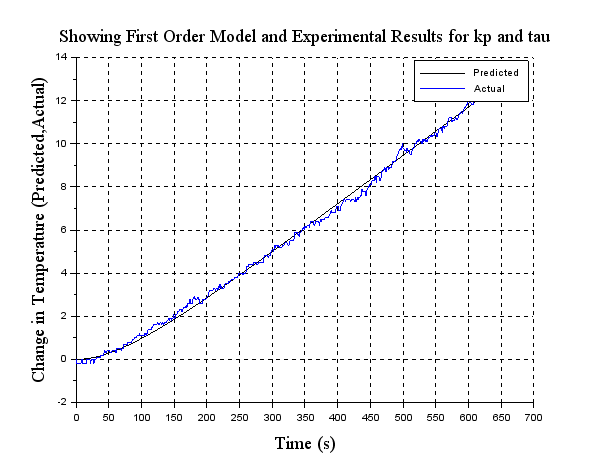
\includegraphics[width=\linewidth]{Ramp-test_manual/ramp-analysis.png}
\caption{Output of the Scilab code {\ttfamily ramp\_virtual.sce}}
\label{firstorder_ramp}
\end{figure} \label{firstorderplot}

\begin{figure} 
\centering
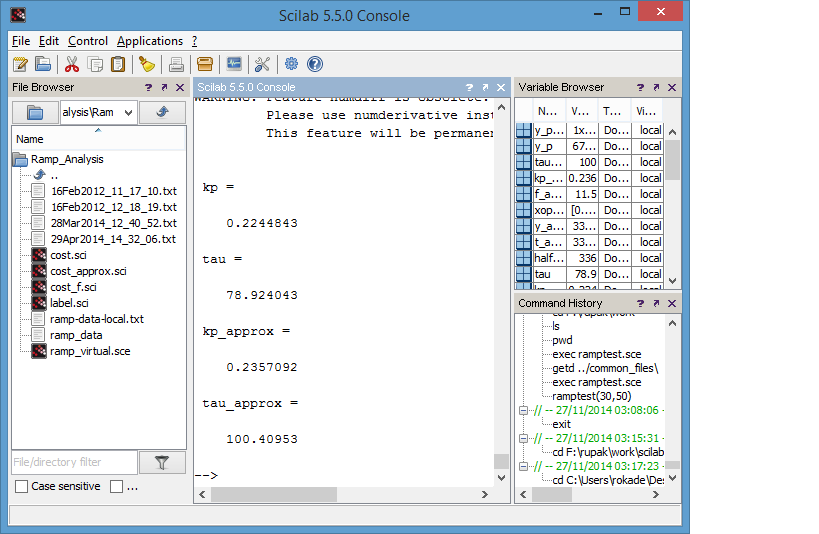
\includegraphics[width=\linewidth]{Ramp-test_manual/ramp-console.png}
\caption{Scilab console after executing code{\ttfamily ramp\_virtual.sce}}
\label{firstorder_ramp_console}
\end{figure} \label{firstorderplot}

\begin{align}
\intertext{The results presented are obtained for the data file {\tt ramp-data-virtual.txt}. This data file is present under the {\tt Ramp\_Test} directory for local experiments. The plot thus obtained is reasonably good. See the Scilab console to get the values of $\tau$ and $K$. It is as shown in figure \ref{firstorder_ramp_console}
The figure \ref{firstorder_ramp} shows a screen shot of the same. We obtain $\tau$ = 78.92, K = 0.22. The transfer function 
obtained here is at the operating point of enterValue percentage of heat. If the experiment is repeated at a different operating point, the transfer function obtained will be different. The gain will correspondingly be more at a higher operating point. This means that the plant is faster at higher temperature. Thus the transfer function of the plant varies with the operating 
point. Let the transfer function we obtain in this experiment be denoted as $G_s$. We obtain}
G_s(s) =  \frac{0.22}{78.92s+1} \label{12}
\end{align}

\section{Discussion}
We summarize our findings now. The experiment has been performed by varying the heater current and keeping the fan 
speed constant. However, the user is encouraged to experiment using different combinations of fan speed 
and heater current. Negative ramp can also be used to make the experiment more informative. 
It is not necessary to keep a particular input constant. For example, you can try giving a ramp input to the 
disturbance signal, i.e., the fan input. The system can also be treated as a second order system. This consideration is necessary as it increases the accuracy of the acquired transfer function \cite{kmm09}.

The necessary codes are listed in the section \ref{rampcodes}.


%###################################
\section{Scilab Code}\label{rampcodes}
\begin{code}
\ccaption{ramp\_test.sci}{\ttfamily ramp\_test.sci}
\lstinputlisting{Scilab/local/Ramp_Test/ramp_test.sci}
\end{code}

\begin{code}
\ccaption{label.sci}{\ttfamily label.sci}
\lstinputlisting{Scilab/Analysis/Ramp_Analysis/label.sci}
\end{code}

\begin{code}
\ccaption{cost.sci}{\ttfamily cost.sci}
\lstinputlisting{Scilab/Analysis/Ramp_Analysis/cost.sci}
\end{code}

\begin{code}
\ccaption{cost\_approx.sci}{\ttfamily cost\_approx.sci}
\lstinputlisting{Scilab/Analysis/Ramp_Analysis/cost_approx.sci}
\end{code}

\begin{code}
\ccaption{ramptest.sci}{\ttfamily ramptest.sci}
\lstinputlisting{Scilab/virtual/RampTest/ramptest.sci}
\end{code}

\begin{code}
\ccaption{ramptest.sce}{\ttfamily ramptest.sce}
\lstinputlisting{Scilab/virtual/RampTest/ramptest.sce}
\end{code}

\begin{code}
\ccaption{ramp\_virtual.sce}{\ttfamily ramp\_virtual.sce}
\lstinputlisting{Scilab/Analysis/Ramp_Analysis/ramp_virtual.sce}
\end{code}


%\bibliography{New} % Adding References
